\chapter{Grundlagen}\label{grundlagen}

% Beispiele Formeln
\[
\begin{gathered}
	y = +1, \text{ falls } \sum_{i=1}^{n} w_i \cdot x_i > b \\
	y = -1, \text{ falls } \sum_{i=1}^{n} w_i \cdot x_i < b
\end{gathered}
\]

\[
qSQI = \begin{cases}
	\text{excellent (E)} & \text{wenn alle 4 } SQI_i \geq 0,9\\
	\text{acceptable (A)} & \begin{cases}
		& \text{wenn 3 der 4 } SQI_i \geq 0,9 \text{ oder}\\
		& \text{wenn alle 4 } SQI_i \geq 0,7 \text{ oder}\\
		& \text{wenn median}(SQI_1, SQI_2, SQI_3) \geq 0,8\\&\text{ }\text{	und } SQI_1 \geq 0,5 \text{ und } SQI_4 \geq 0,7
		\end{cases}\\
	\text{untrustworthy (U)} & \text{sonst}\\
\end{cases}
\]

% Beispiel figure

\begin{figure}[H]
	\centering
		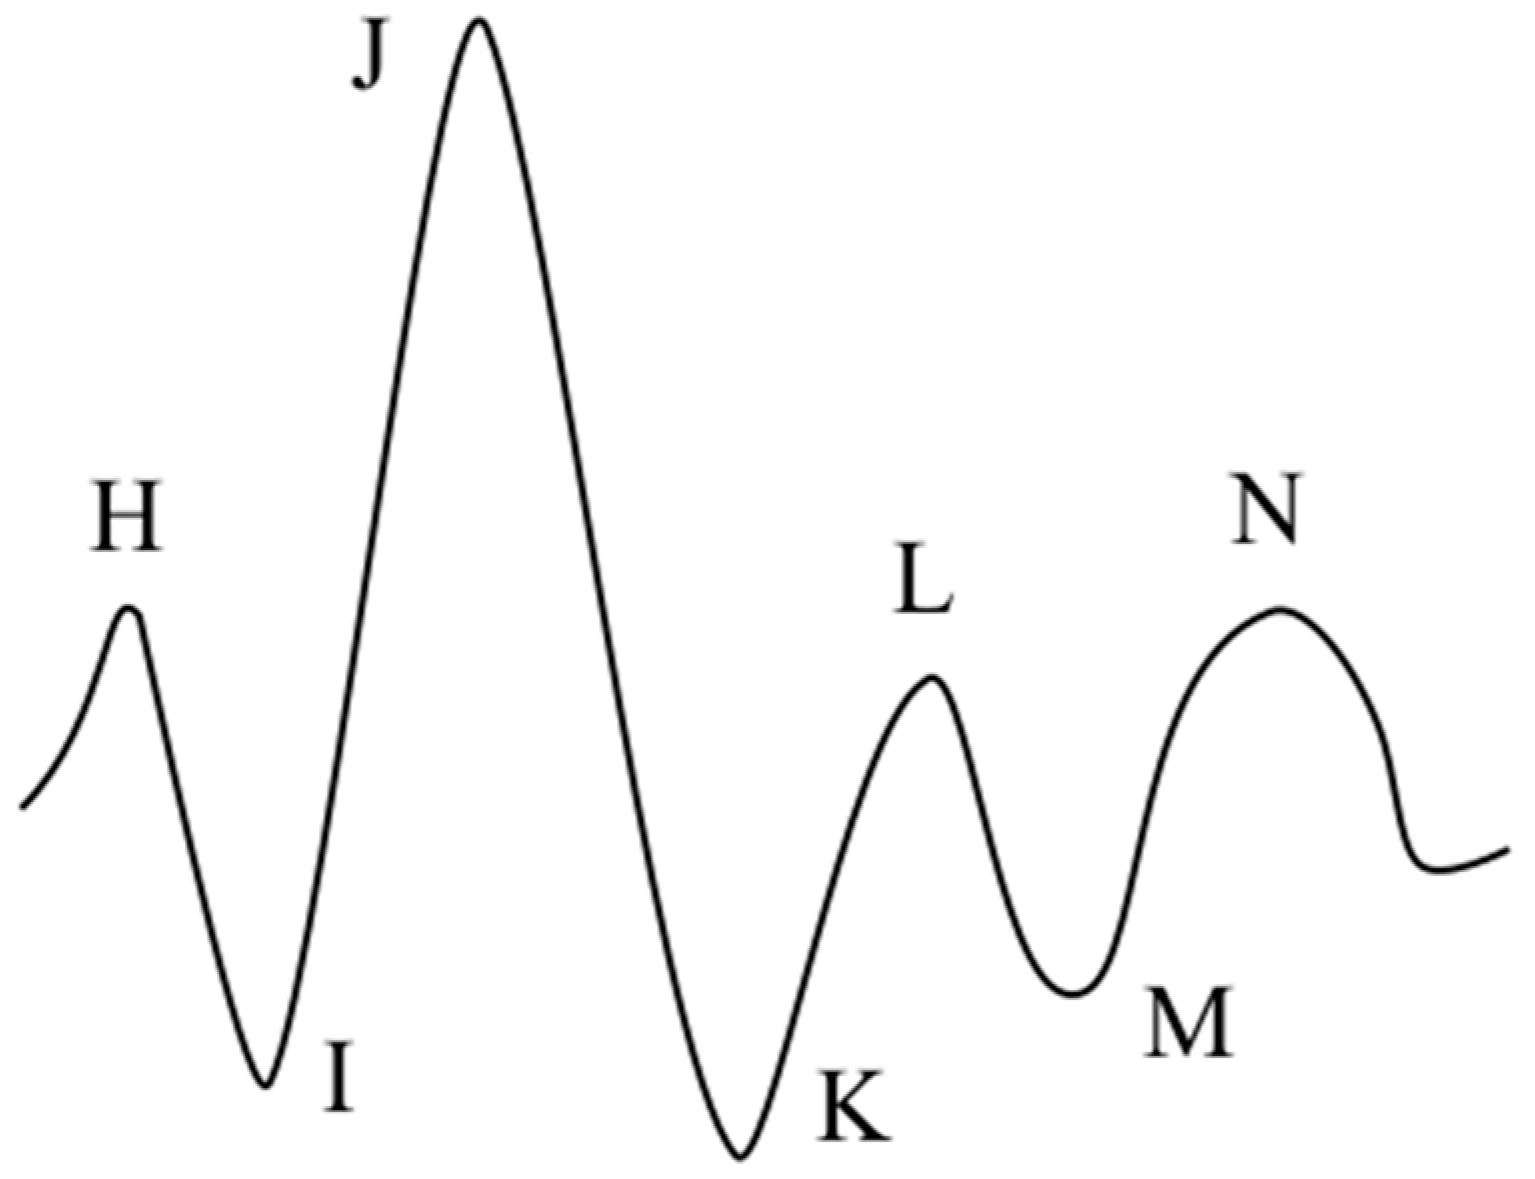
\includegraphics[width=0.7\textwidth]{pic/bcgWaveform.png}
	\caption[Beispiel eines typischen \ac{BKG}-Signals mit Nomenklatur]{Beispiel eines typischen \ac{BKG}-Signals mit Nomenklatur\protect\footnotemark}
	\label{fig:bcgwaveform}
\end{figure}
\footnotetext{Entnommen aus \cite{Albukhari2019} nach \cite{Starr1939}.}
